\documentclass[
    12pt, % Default font size, values between 10pt-12pt are allowed
    %spanish, % Uncomment for Spanish
]{fphw}

% Template-specific packages
\usepackage[T1]{fontenc} % Output font encoding for international characters
\usepackage{fontspec,unicode-math} % Required for using utf8 characters in math mode
\usepackage{parskip}  % To add extra space between paragraphs
% \usepackage{mathpazo} % Use the Palatino font
\usepackage{graphicx} % Required for including images
\usepackage{booktabs} % Better horizontal rules in tables
\usepackage{hyperref} % For links (both internal and external)
\usepackage{listings} % Required for insertion of code
\usepackage{enumerate}% To modify the enumerate environment
\usepackage{cleveref} % Better \ref command -> \cref
\usepackage{import}   % This 4 packages and the command allow importing pdf
\usepackage{xifthen}  % figures generated with inkscape
\usepackage{pdfpages} % Source: https://castel.dev/post/lecture-notes-2/
\usepackage{amsthm}   % Mathematical environments
\usepackage{mathtools}% Mathematical environments
\usepackage{relsize}  % \smaller and \mathsmaller commands
\usepackage{physics}  % A lot of good commands for mathematics
\usepackage{multirow}
\usepackage{appendix}
\usepackage[binary-units]{siunitx}  % To write magnitudes with units
\usepackage{transparent}
\newcommand{\incfig}[1]{%
    \def\svgwidth{0.95\columnwidth}
    \small
        \import{./images/}{#1.pdf_tex}
}

\setlength{\parindent}{15pt}

%----------------------------------------------------------------------------------------
%    ASSIGNMENT INFORMATION
%----------------------------------------------------------------------------------------

\title{Assignment 2 \\
Introduction to vectorization and parallelization} % Assignment title

\author{Emilio Domínguez Sánchez} % Student name

\date{November 16th, 2020} % Due date

\institute{University of Murcia \\ Faculty of Informatics} % Institute or school name

\class{Arquitectura y Organización de Computadores} % Course or class name

\professor{Dr. José Manuel García Carrasco} % Professor or teacher in charge of the assignment

%----------------------------------------------------------------------------------------
%    Definitions
%----------------------------------------------------------------------------------------

\newtheorem{theorem}{Informal Theorem}
\lstset{
    language=C++,
    basicstyle=\scriptsize,        % the size of the fonts that are used for the code
    frame=L,
    captionpos=t,
    numbers=left,
    numbersep=10pt,
    breaklines=true,
    stepnumber=1,
    escapeinside={/*}{*/},
    showlines=true,
}
\setlength{\headheight}{22.77pt}
\newcommand{\tech}{\texttt}
\newcommand{\gcc}{\textit{gcc}}
\newcommand{\clang}{\textit{clang}}
\newcommand{\icc}{\textit{icc}}
\newcommand{\OpenMp}{\textit{OpenMp}}

\begin{document}

\maketitle % Output the assignment title, created automatically using the information in the custom commands above

%----------------------------------------------------------------------------------------
%    ASSIGNMENT CONTENT
%----------------------------------------------------------------------------------------

\section*{Instructions for the student}

    You are asked to write a document where you
explain breefly the positive aspects of the assignment,
as well as the negatives and
anything that you may have missed in it.

\noindent
In addition, you should answer the following questions.

\noindent
The length of the document shall be kept between $700$ and $1000$ words and
the inclusion of graphics will be graded positively.

\section*{Questions}

\subsection*{Exercise 1: Vectorization}

\begin{enumerate}
    \item For each loop in the given program,
    identify the dependencies between iterations and explain how they would
    affect the compiler's vectorization.

    \item Using the already known server, compile the program with the command

    \begin{lstlisting}[gobble=8]
        icc -std=c++11 -Wall -O2 -xCORE-AVX2
                -qopt-report -qopt-report-file=file.optrpt
    \end{lstlisting}

    and explain, looking at the vectorization report,

    \begin{enumerate}
        \item which loops have been vectorized and
        if the compiler had to do any transformations to do so.

        \item which loops have not been vectorized but there exist manual transformations that would allow it.
    \end{enumerate}
\end{enumerate}

\subsection*{Exercise 2: Parallelization}

\begin{enumerate}
    \item Identify the loops of the main routine of the algorithm and
    analyse if they could be the target of parallelization.
    Include the \OpenMp{} \tech{\#pragma}s that would be necessary to parallelize them.

    \item Parallelize each of the parallelizable loops,
    first independently and then at the same time.
    For each possibility, measure the run time with the $3$ data sets provided.
    You are free to use your own hardware.
\end{enumerate}

%----------------------------------------------------------------------------------------

\section{Data Hazards and Vectorization}

\subsection{Original Code}

\begin{lstlisting}[gobble=4]
    #include <iostream>

    using namespace std;

    constexpr int iterations = 100;
    constexpr int arrays_size = 1000000;

    double A[arrays_size];
    double B[arrays_size];
    double C[arrays_size];

    int main(int argc, char** argv) {
      double total = 0;

      for (int i = 0; i < iterations; ++i) {
        for (int i = 0; i < arrays_size-1; ++i) {
          A[i] = i*2/3;
          B[i+1] = A[i]-B[i];
        }

        for (int i = 0; i < arrays_size-1; ++i) {
          A[i] = A[i]-B[i];
          B[i+1] = 2*C[i];
        }

        for (int i = arrays_size-1; i > 0; --i) {
          A[i-1] = A[i]+C[i];
          B[i] = C[i]-B[i];
        }

        for (int i = 0; i < arrays_size; ++i) {
          C[i] = A[i]+2*B[i];
        }

        for (int i = 0; i < arrays_size; ++i) {
          total += C[i];
        }
      }

      cout << total << endl;
      return 0;
    }
\end{lstlisting}

\subsection{Analysis}

\subsubsection{Outer Loop}

\begin{lstlisting}[gobble=4]
    for (int i = 0; i < iterations; ++i) {
      for /*$\ldots$*/
      for /*$\ldots$*/
      for /*$\ldots$*/
      for /*$\ldots$*/
      for /*$\ldots$*/
    }
\end{lstlisting}

    There is no point in vectorizing the outer loop because it contains multiple inner loops;
inner loops that even depend one upon the next.
The vectorization can happen inside the inner loops though.

\newpage

\subsubsection{First Inner Loop}

\begin{lstlisting}[gobble=4]
    for (int i = 0; i < arrays_size-1; ++i) {
      A[i] = i*2/3;
      B[i+1] = A[i]-B[i];
    }

\end{lstlisting}

    The first inner loop presents two operations.
The first one only depends on the loop variable, \tech{i}.
The loop variable changes at the end of each iteration and
could seem like a data hazard for vectorization, but in reality
the change of the variable is determined and does not depend on the input of the program.
In fact, a standard compiler can easily unroll the loop (\cref{fig:loop-variable-unroll}).
Therefore it is easily parallelizable.
However, the second operation sets the value of the variable \tech{B[i+1]},
that will be used by this operation in the next iteration.
This will affect the automatic vectorization (making it impossible),
because it tries to operate on the current value and the following directly,
but the latter depends on the former.

\begin{figure}[h]

    \caption{How compilers can unroll assignments over the loop's variable}
    \label{fig:loop-variable-unroll}

    \begin{minipage}[t][8cm][t]{.45\textwidth}

        \begin{lstlisting}[gobble=12,title=Original code]
            for (int i = 0; i < arrays_size; ++i) {
              A[i] = f(i);
            }

        \end{lstlisting}

        \vfill

        In the previous code, $f$ is a function in the mathematical sense.
        It is an expression that involves the variable $i$, but not a function call.
        You can imagine that it was an inlined procedure.

        \vfill

        In the right code, the loop has been unrolled and the compiler can
        group the set of $k$ operations inside it as a single vectorized operation.

    \end{minipage}
    \hfill
    \begin{minipage}[t][8cm][t]{.45\textwidth}

        \begin{lstlisting}[gobble=12,title=Unrolled code]
            int mod = arrays_size%k;
            switch(mod) {
                case k-1:
                    A[k-1] = f(k-1);
                case k-2:
                    A[k-2] = f(k-2);
                /*$\ldots$*/
                case 2:
                    A[2] = f(2);
                case 1:
                    A[1] = f(1);
            }
            for (int i = mod; i < arrays_size; i+=k) {
              A[i] = f(i);
              A[i+1] = f(i+1);
              /*$\ldots$*/
              A[i+k-2] = f(i+k-2);
              A[i+k-1] = f(i+k-1);
            }

        \end{lstlisting}

    \end{minipage}

\end{figure}

    However, it is possible to program the loop in a way that is vectorizable.
The values stored in \tech{B} are a reduction of the array \tech{A}.
%
\begin{equation*}
    \tech{B[i+1]} = \tech{A[i]}-\tech{A[i-1]}+\tech{A[i-2]}-
        \ldots+(-1)^i(\tech{A[0]}-\tech{B[0]}).
\end{equation*}
But the values of the array \tech{A} are determined by $i$.
The following code uses a formula I derived from the series\footnote{
    You can prove by induction that the reduction over \tech{A} is equal to \tech{(i+1)/3}
    when \tech{B[0]} is zero.
    The process is omitted since it is not of much interest.
} to find the values for \tech{B[i]},
and the \icc{} compiler is capable of vectorizing it.

\begin{lstlisting}[gobble=4]
    for (int i = 0; i < arrays_size-1; ++i) {
        A[i] = i*2/3;
        // We could omit the rhs since B[0] == 0 throughout the program
        // But let's try to keep the initial semantics.
        B[i+1] = (i+1)/3 + (1-2*(i&1))*B[0];
    }

\end{lstlisting}

\subsubsection{Second Inner Loop}

\begin{lstlisting}[gobble=4]
    for (int i = 0; i < arrays_size-1; ++i) {
      A[i] = A[i]-B[i];
      B[i+1] = 2*C[i];
    }

\end{lstlisting}

    The second loop presents a similar problem to the first one.
The second operation, \tech{B[i+1] = 2*C[i]} sets the value of a variable
that is needed in the next iteration for the first operation.
However, the result of the assignment is
independent of the variables modified inside the loop
because it is \tech{2*C[i]}
(if we assume \tech{C} does not share memmory adresses with \tech{A} or \tech{B}).
A clever compiler (or programmer) could rewrite the code as

\begin{lstlisting}[gobble=4]
    A[0] = A[0] - B[0];
    B[1] = 2*C[0];
    for (int i = 1; i < arrays_size-1; ++i) {
      A[i] = A[i]-2*C[i-1];
      B[i+1] = 2*C[i];
    }

\end{lstlisting}

\noindent
or even simpler, as

\begin{lstlisting}[gobble=4]
    A[0] = A[0] - B[0];
    B[arrays_size-1] = 2*C[arrays_size-2];
    for (int i = 1; i < arrays_size-1; ++i) {
      A[i] = A[i]-2*C[i-1];
      B[i] = 2*C[i-1];
    }

\end{lstlisting}

    At first I thought the compiler would not be smart enough
to reason like this and parallelize the loop.
To my surprise
    , as we will see later in the parallelization report
(\cref{lst:vectorization-report}),
it happens that the compiler realized that it was possible to do a simpler transformation:
swapping the order of the operations.
I said this loop was similar to the first one,
but the difference is that the dependency is now between different operations,
one operation waits for the result of the other.
Therefore, if we can vectorize both operations,
all of the values of the second operation would depend on the previous vectorized operation,
instead of depending one upon another.

\subsubsection{Third Inner Loop}

\begin{lstlisting}[gobble=4]
    for (int i = arrays_size-1; i > 0; --i) {
      A[i-1] = A[i]+C[i];
      B[i] = C[i]-B[i];
    }

\end{lstlisting}

    The third loop posses a similar data hazard as that seen in the first loop.
The first operations assigns to \tech{A[i-1]} which is also used in the following iteration.
As before, we cannot expect the compiler to optimize this loop.

    Note that the result of the operations over the array \tech{A} is

\begin{equation*}
    \text{\tech{A}}[i] = \text{\tech{A}}[\operatorname{arrays\_size}-1] +
        \sum_{j=i+1}^{\operatorname{arrays\_size-1}} \text{\tech{C}}[j].
\end{equation*}

\noindent
    With this expression, we have eliminated the dependency on \tech{A},
and I believe most compilers are able to do simplifications like this one.
However, the sum reduction over \tech{C} still makes it very difficult to vectorize this loop.
And although later we will see a loop that finds the sum over an array and is vectorized,
we cannot use the same technique here.
This case is different because we need to store the value of the sum at each iteration.

\subsubsection{Fourth Inner Loop}

\begin{lstlisting}[gobble=4]
    for (int i = 0; i < arrays_size; ++i) {
      C[i] = A[i] + 2*B[i];
    }

\end{lstlisting}

    The fourth loop is the first example of a loop that is trivially vectorizable
because it does not contain any data hazards.

\subsubsection{Fifth Inner Loop}

\begin{lstlisting}[gobble=4]
    for (int i = 0; i < arrays_size; ++i) {
      total = total + C[i];
    }

\end{lstlisting}

    The fifth loop is a sum reduction of the array \tech{C}.
In this type of loops, the only data hazard is that
the next iteration cannot be performed (just as is written)
without having the result of the previous one.
However, when the opeartion is conmutative, as is the case,
we can sum over many variables and then add them.
That is, the loop could be transformed to

\begin{lstlisting}[gobble=4]
    for (int i = 0; i < arrays_size; i+=k) {
      total0 = total0 + C[i];
      total1 = total1 + C[i+1];
      /*$\ldots$*/
      totalkm1 = totalkm1 + C[i+k-1];
    }
    total = total0 + /*$\ldots$*/ + totalkm1;

\end{lstlisting}

\noindent
which can be easily vectorized when there are enough variables to fill a vector.

\subsection{Vectorization performed by \icc}

    If we compile with the flags \tech{-qopt-report -qopt-report-file=<file>}
with the compiler \icc{},
we can get a vectorization report for each loop in our program.
You can see the report for our code in \cref{lst:vectorization-report}.

\newpage
\begin{lstlisting}[
    gobble=4,
    caption=Vectorization Report,
    label=lst:vectorization-report,
]
    Begin optimization report for: main(int, char **)

        Report from: Interprocedural optimizations [ipo]

    INLINE REPORT: (main(int, char **)) [1] loops.cpp(12,33)
      -> (42,8) std::basic_ostream<char, std::char_traits<char>>::operator<<(std::basic_ostream<char, std::char_traits<char>> *, double)
      -> (42,17) std::basic_ostream<char, std::char_traits<char>>::operator<<(std::basic_ostream<char, std::char_traits<char>> *, std::basic_ostream<char, std::char_traits<char>>::__ostream_type &(*)(std::basic_ostream<char, std::char_traits<char>>::__ostream_type &))


        Report from: Loop nest, Vector & Auto-parallelization optimizations [loop, vec, par]


    LOOP BEGIN at loops.cpp(15,3)
       remark #15542: loop was not vectorized: inner loop was already vectorized

       LOOP BEGIN at loops.cpp(17,5)
          remark #15344: loop was not vectorized: vector dependence prevents vectorization. First dependence is shown below. Use level 5 report for details
          remark #15346: vector dependence: assumed FLOW dependence between  line 19 and  line 19
       LOOP END

       LOOP BEGIN at loops.cpp(22,5)
          remark #25427: Loop Statements Reordered
          remark #15300: LOOP WAS VECTORIZED
       LOOP END

       LOOP BEGIN at loops.cpp(27,5)
          remark #15344: loop was not vectorized: vector dependence prevents vectorization. First dependence is shown below. Use level 5 report for details
          remark #15346: vector dependence: assumed FLOW dependence between  line 28 and  line 28
          remark #25438: unrolled without remainder by 2  
       LOOP END

       LOOP BEGIN at loops.cpp(32,5)
          remark #15300: LOOP WAS VECTORIZED
       LOOP END

       LOOP BEGIN at loops.cpp(36,5)
          remark #15300: LOOP WAS VECTORIZED
       LOOP END

       LOOP BEGIN at loops.cpp(22,5)
       <Remainder loop for vectorization>
          remark #25436: completely unrolled by 3  
       LOOP END
    LOOP END
    ===========================================================================

    Begin optimization report for: __sti__$E()

        Report from: Interprocedural optimizations [ipo]

    INLINE REPORT: (__sti__$E()) [9] <compiler generated>

    ===========================================================================
\end{lstlisting}

    The vectorization shows results similar to what we expected.
The first and third inner loops,
which we saw presented very similar problems,
were not vectorized.
The second loop was vectorized by swapping the order of the operations, as we already saw.
And the loop with the reduction was also vectorized.

% \section{Extra: Additional thought on vectorizing}

%     I want to write here what can I see as the principal theorem of vectorization.
% I write it because I have seen that it is sometimes believed that
% we can loose performance vectorizing.
% This idea comes from the belief that we would need to 

% \begin{theorem}
%     Given a loop $l$ of the form

%     \begin{lstlisting}[gobble=8]
%         i ← i_0

%         loop:
%         // Set of assembly instructions without
%         // dependencies with the following iterations
%         ins0(vars, %i)
%         ins1(vars, %i)
%         /*$\ldots$*/
%         insn(var, %i)

%         i ← i + 1
%         // Comparison of i and an integer (resp. expression)
%         // that is whose value does not change at any moment
%         // inside the loop
%         cmp i <end condition>
%         jne loop

%     \end{lstlisting}

%     it is always possible to vectorize the loop and the performance,
%     when measured on a machine model with uniform memory (no cache misses and such)
%     and an infinite amount of vector registers.
% \end{theorem}
% \begin{proof}
%     Let $v$ be the number of variables that fit into a vector.
%     Rewrite the loop to be

%     \begin{lstlisting}[gobble=8]
%         // preinitizalize vectors
%         //    Vector vi
%         vi ← [i_0 i_0+1 /*4\ldots*/ i_0+v-1]
%         //    Vectors of immediates used in the instructions
%         //      Incremet vector
%         vinc ← [v v /*$\ldots$*/ v]

%         // Operate on the first iterations of the loop
%         // when the loop length is not a multiple of /*$v+1$*/

%         loop:
%         vectorized ins0(vars, %vector vi)
%         vectorized ins1(vars, %vector vi)
%         /*$\ldots$*/
%         vectorized insn(vars, %vector vi)

%         vi ← vi + vinc
%         cmp i0 <end condition>
%         jne loop

%     \end{lstlisting}
% \end{proof}

% \begin{lstlisting}[gobble=4]
%     for (int i = 0; i < arrays_size-1; ++i) {
%       A[i] = i*2/3;
%       B[i+1] = A[i]-B[i];
%     }

% \end{lstlisting}


\section{Extra: Additional thoughts on loops transformations}

    I want to cover a topic related to vectorization.
And that topic is to not forget about the pipeline when we think about vectorization.
Let us base our example in the last loop of the previous exercise.

\begin{lstlisting}[gobble=4]
    // Pre processed
    for (int i = 0; i < arrays_size; ++i) {
      total = total + C[i]
    }

    // Post processed
    for (int i = 0; i < arrays_size; i+=k) {
      total0 = total0 + C[i];
      total1 = total1 + C[i+1];
      /*$\ldots$*/
      totalkm1 = totalkm1 + C[i+k-1];
    }
    total = total0 + /*$\ldots$*/ + totalkm1;

\end{lstlisting}

    Note that the only property that the reduction operation needs to have
to perform this transformation is \textit{conmutativity}.
Conmutativity lets us use multiple variables instead of one,
which makes it possible to vectorize.
Therefore, a natural question arises: how many variables should we use?
I believe a typical pitfall is thinking that as many as fit into a vector.
If we just use as many variables as fit into a vector,
then we have increased our performance,
because now each time we emit an operation we perform the equivalent to many
(even though the latency for vectorized operations is usually slightly bigger).
But we still have a similar problem as before, each vectorized operation depends on
the previous one and we cannot fill the pipeline completely.
For example, in my computer the latency for floating point additions and
floating point vector additions, which account for $4$ traditional additions,
are $\SI{3}{\ms}$ and $\SI{5}{\ms}$ respectively.
The original code would perform $1$ operation every $\SI{3}{\ms}$,
and the improved code with $4$ variables into the same vector would perform
$4$ operations every $\SI{5}{\ms}$ which is $4\cdot \frac{3}{5} = 2.4$ times more.
But if we used $20$ variables\footnote{
    In general, the number of variables that fit into a vector times
    the latency of the vectorized operation.
}
distributed among $5$ vectors,
we would be able to emit one vectorized operation per millisecond,
resulting in an increase of $4 \cdot 3 = 12$ times in performance
comparing to the original code or $5$ times
comparing to the poorly vectorized option\footnote{
    I have checked the assembly myself and this is indeed
    what the compiler is doing.
}.
But the story does not end there.
Using multiple variables to fill the pipeline with traditional additions
would give us $3$ times better performance,
which is \textbf{more that what we achieved by vectorizing} the wrong way!

    The important takeaway is that it is more important\footnote{
    I am arguing comparing the latencies of my hardware,
    but in general, as far as I have seen,
    it holds for most hardware typical values.
} to fill the pipeline than it is to vectorize.
Furthermore, the transformations that erase the dependencies in a loop
make it easier not only to fill the pipeline or vectorize it,
but also to parallelize it automatically.
Hence, we should seek to make this transformations or
make it easier for the compiler to recognize that it can do them.

\newpage

\section{Parallelization}

\subsection{Extract of the Original Code}

\begin{lstlisting}[gobble=4]
    void solve(
      Matrix<double>& state,
      double tolerance,
      int& iterations,
      double& last_difference
    ) {
      Matrix<double> next_state = state;
      iterations = 0;
      double difference;
      do {
        difference = 0;
        for (size_t i = 1; i < state.height - 1; ++i) {
          for (size_t j = 1; j < state.width - 1; ++j) {
            next_state[i][j] = (state[i][j]
                                + state[i + 1][j + 1]
                                + state[i - 1][j + 1]
                                + state[i + 1][j - 1]
                                + state[i - 1][j - 1]) / 5;
            difference = max(difference, abs(next_state[i][j] - state[i][j]));
          }
        }

        state.swap_data(next_state);

        if (verbose) {
          cout << "Iteration " << iterations << ":\n" << state;
          cout << "Difference: " << difference << endl;
        }
        ++iterations;
      } while (difference > tolerance);
      last_difference = difference;
    }

\end{lstlisting}

\subsection{Analysis}

    The function \tech{solve} consists of three loops.
The outer one is run until the values stabilize.
Because at each iteration it needs to work with the matrix of the previous iteration,
this loop is hardly parallelizable.
The two inner loops set the values of the matrix \tech{next\_state}
according to the values of \tech{state} and then swap both.
In this case, the matrix \tech{state} is not modified inside the loops and can be
treated as an inmutable object
(which means that it can be shared between threads).
Therefore, the update of the matrix \tech{next\_state} is what would be called
an \textit{embarrassingly parallelizable} procedure.
The only problem is updating the variable \tech{difference},
which is a reduction variable over \tech{next\_state} and \tech{state}.
The solution is simple, to work with independent variables in each thread
and then to take the maximum of them all.
\OpenMp{} implements a directive called \textit{reduce} to perform this task.

\subsection{Parallelizing the outer loop}

\begin{lstlisting}[gobble=4]
    #pragma omp parallel for reduction(max:difference)
    for (size_t i = 1; i < state.height - 1; ++i) {
      for (size_t j = 1; j < state.width - 1; ++j)

\end{lstlisting}

    Parallelizing the first loop gives very good results.
The results (\cref{fig:parallelization-results}) show a proportional improvement
as the number of threads gets close to $4$, the number of cores in my hardware.
After that, we see an increase in time in all cases if we use $5$ cores.
And that value decreases a little when we use $6$ or $7$,
until it is the same it was with $4$ when we use $8$ cores.

    First, it is clear that we cannot
obtain better performance using simultaneous multi-threading.
The problem is not in the memmory because the even the biggest
test is only $\SI{1.3}{\mebi\byte}$,
which fits completely in a L3 cache.
Therefore, we conclude that our application can fill the pipeline.
My interpretation is that the increase in time when using $5$ cores
comes from the fact that either the $2$ threads share a core and
the others work on a single core,
or all of the threads share the $4$ cores, which could lead to cache misses.
And I believe that if it was the latter case,
then when we used $8$ threads the two same threads would probably
be run in the same core by the operating system.

\begin{figure}[h]
    \centering
    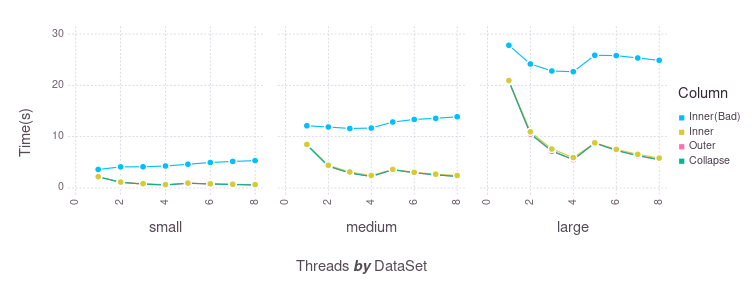
\includegraphics[width=0.98\textwidth]{prac2/times-plot.png}
    \caption{Execution times by test and optimization}
    \label{fig:parallelization-results}
\end{figure}

    If it were the first case, though,
the threads that are scheduled together would need twice the time to complete
comparing to using $4$ theads, because the pipeline is filled.
But the amount of work they need to complete if the scheduling is static is
$\frac{4}{t}$ of the previous amount, where $t$ is the number of threads.
Therefore, we would see an increase in propotional to $2\frac{4}{t} = \frac{8}{t}$.
I have compared the real values with the theoretical values in \cref{tab:hypothesis-check},
showing that this hypothesis is very plausible.

\begin{table}[h]
    \centering
    \renewcommand{\arraystretch}{1.5}
    \begin{tabular}{p{2cm}l ||ccccc}
        && \multicolumn{5}{c}{\textbf{Number of Threads (Hypothetic value)}} \\
        \textbf{Testcase} && 4 ($x$) & 5 ($\frac{8}{5}x$) & 6 ($\frac{8}{6}x$)
            & 7 ($\frac{8}{7}x$) & 8 ($\frac{8}{8}x$) \\
        \hline\hline
        \multirow{2}{*}{\textbf{Small}}
        & Hypothetic Value & \multirow{2}{*}{$0.59$} & $0.94$
            & $0.79$ & $0.67$ & $0.59$ \\
        & Measured Value & & $0.92$ & $0.77$ & $0.67$ & $0.59$ \\
        \hline
        \multirow{2}{*}{\textbf{Medium}}
        & Hypothetic Value & \multirow{2}{*}{$2.25$} & $3.60$
            & $3.00$ & $2.57$ & $2.25$ \\
        & Measured Value & & $3.56$ & $2.97$ & $2.55$ & $2.26$ \\
        \hline
        \multirow{2}{*}{\textbf{Large}}
        & Hypothetic Value & \multirow{2}{*}{$5.52$} & $8.83$
            & $7.36$ & $6.31$ & $5.52$ \\
        & Measured Value & & $8.79$ & $7.36$ & $6.31$ & $5.56$ \\
    \end{tabular}
    \caption{Time predicted when the schedule is static and
    the threads always run in the same core versus the measured time.}
    \label{tab:hypothesis-check}
\end{table}

\subsection{Parallelizing the inner loop}

\begin{lstlisting}[gobble=4]
    #pragma omp parallel reduction(max: difference)
    {
      for (size_t i = 1; i < state.height - 1; ++i) {
        #pragma omp for nowait
        for (size_t j = 1; j < state.width - 1; ++j) {
          next_state[i][j] = (state[i][j]
                              + state[i + 1][j + 1]  
                              + state[i - 1][j + 1]  
                              + state[i + 1][j - 1]  
                              + state[i - 1][j - 1]) / 5;
          difference = max(difference, abs(next_state[i][j] - state[i][j]));
        }
      }
    }

\end{lstlisting}

    Parallelizing the second loop is generally a worse option.
In our case, it requires more reasoning to get a better performance with \OpenMp{}.
If we use the pragma \tech{\#pragma omp parallel for reduction(max: difference)}
just before the second loop,
we are introducing the hassle of scheduling the distinct threads,
the join operation\footnote{
    The threads wait at the end of a \textit{parallel for} until all of them are done.
    The point in the code where a set of threads waits until the rest are ready
    is often referred as a \textit{barrier}.
} and the atomic operation associated with the reduction
in each iteration of the outer loop.
But it is not necessary to perform that work at the end of each outer iteration
because there are no dependencies between the iterations of the inner loop.
The correct way to perform this parallelization is to
create the parallel zone before the first loop and
divide the second loop between the threads.
The directive \tech{nowait} removes the \textit{barrier} at the end of the inner loop.
The threads join at the end of the parallel zone, both of the loops, instead.
This amortizes the overhead of the parallelism over many iterations.

    I decided to include the results of the worse parallelization too
(\cref{fig:parallelization-results}).
In that case, the improvement is scarce or, for small cases, there is even penalization.
While with the correct one the results are very close to what we obtained
parallelizing the outer loop.

\subsection{Combined parallelization}

\begin{lstlisting}[gobble=4]
    #pragma omp parallel for reduction(max:difference) collapse(2)
    for (size_t i = 1; i < state.height - 1; ++i) {
      for (size_t j = 1; j < state.width - 1; ++j)
\end{lstlisting}

    \OpenMp{} offers an option to collapse rectangular loops and parallelize the corresponding
one-dimensional loop.
With this the threads are managed once for every matrix update.
This optimization is useful to make it easier to balance the load\footnote{
    The balance of the load can be distributed statically,
    generating code that divides the number of iterations proportionally to each thread.
    But the balance can also be distributed dynamically, depending on the progress of each thread.
    Because in practice, even if all the tasks are the same,
    the access to cache and memmory can make some threads work slower.
    For this type of application though, static scheduling is probably the best.
} on each thread when the number of rows in the matrix is close to the number of threads.
As it is not the case, we did not expect an improvement in run time.
\Cref{lst:parallelization-results} shows identical results to parallelizing the outer loop.

\newpage

\begin{appendices}

\section*{Appendices}

\section{Time dataset}

\lstinputlisting[
    caption=Values used in \cref{fig:parallelization-results}.,
    label=lst:parallelization-results,
    stepnumber=0,
]{prac2/heat.all.tsv}

\end{appendices}

%----------------------------------------------------------------------------------------

\end{document}
